\chapter{Implementation}
\label{ch:implement}

This chapter covers the implementation based on the HMModelers workflow. First, the processing of input data by including secondary structure data is described. This is followed by a description of the adaptation of the \ac{pHMM} and of the scoring algorithms. This section focuses on the modifications made in HMModeler. More information on HMModeler and its other implementations can be found in \cite{Graf.2011, MathiasOberkirchner.2014, Mayer.2014}.

\section{HMModeler}

HMModeler is a software package for protein classification jointly developed by researchers at the Salzburg University of Applied Sciences and the University of Salzburg. 
Although HMModeler was designed as an extension for UCSF Chimera\footnote{UCSF Chimera \url{https://www.cgl.ucsf.edu/chimera/} (accessed July 18, 2018).}, the current version runs independently with its own \ac{GUI}. The core of HMModeler is written in Python, while time-consuming algorithms are also implemented with faster C++ libraries. The  web-based \ac{GUI} communicates with the core system via RESTful\footnote{Representational State Transfer (REST) is an architectural paradigm for communication between distributed machines or applications.} web services. HMModeler is platform-independent and runs both on Windows and Linux operating systems. 
The program uses the Smith-Watermann-style variant of \ac{pHMM}, shown in Figure \ref{fig:pHHMsw}. This variant is used for local alignments, by using flanking states with transitions from the beginning to each match state as start-model, and from each match state to the end state as end-model. 

The \ac{GUI} allows skilled experts to introduce prior information about the targeted protein family into the \ac{HMM}. In particular, the user can interactively define parts of the protein with increased or decreased insertion and deletion probabilities. The user can also modify the extent to which the emission probabilities in the single-model columns of the \ac{pHMM} are extracted. This can be done purely through the given \ac{MSA}; alternatively, the probabilities are determined from a priori distributions.
Finally, the user can define so-called expert sets that override other estimation methods and set the possible emissions in certain model states to an explicit set of amino acids. Currently, the software only uses the primary structure for building the \ac{pHMM} and scores sequences against it with the Viterbi and forward algorithms.
 



\begin{figure}[H]
	\begin{center}
		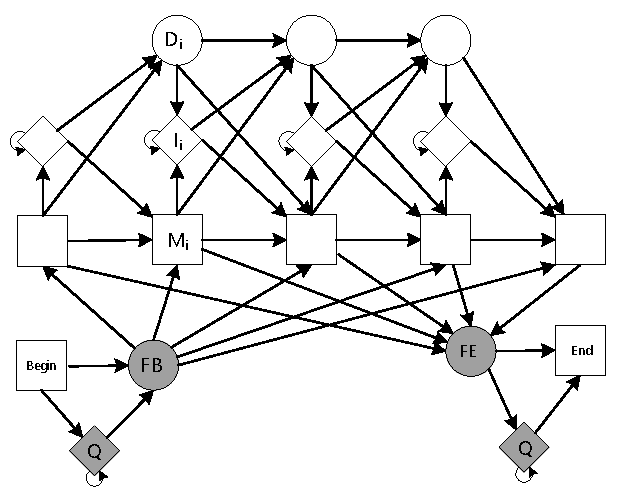
\includegraphics[width=0.78\textwidth]{fig/pHMMsw}
	\end{center}
	\caption[Smith-Waterman variant of a \acs{pHMM}.]{Smith-Waterman variant of a \acs{pHMM}, adapted from \cite{Durbin.1998}.}
	\label{fig:pHHMsw}
\end{figure}

\section{Input Data}
\label{sec:inputData}

First, HMModeler takes an \ac{MSA} as input to train its \ac{pHMM}. HMModeler can process files in the \textit{Stockholm} file format, uploaded by the user or referenced by a project ID from the multiple structure alignment Server PIRATES\footnote{Multiple structure alignment server PIRATES: \url{https://biwww.che.sbg.ac.at/pirates} (accessed July 18, 2018).}. 

The Stockholm format is a markup format for \ac{MSA}, where each sequence can be annotated with additional features, such as the corresponding secondary structure for each amino acid residue. The definition of the Stockholm format can be found in \cite{Sonnhammer.xxx}. 

Figure \ref{fig:flowReadMSA} shows the workflow implemented for determining the secondary structure. First, all sequences in the \ac{MSA} are read. 
If no structure information is provided for one or more sequences, the secondary structure is retrieved from the \ac{PDB} or predicted using the MetaSSPred method (see Section \ref{sec:BSSP}).

\begin{figure}[ht]
	\begin{center}
		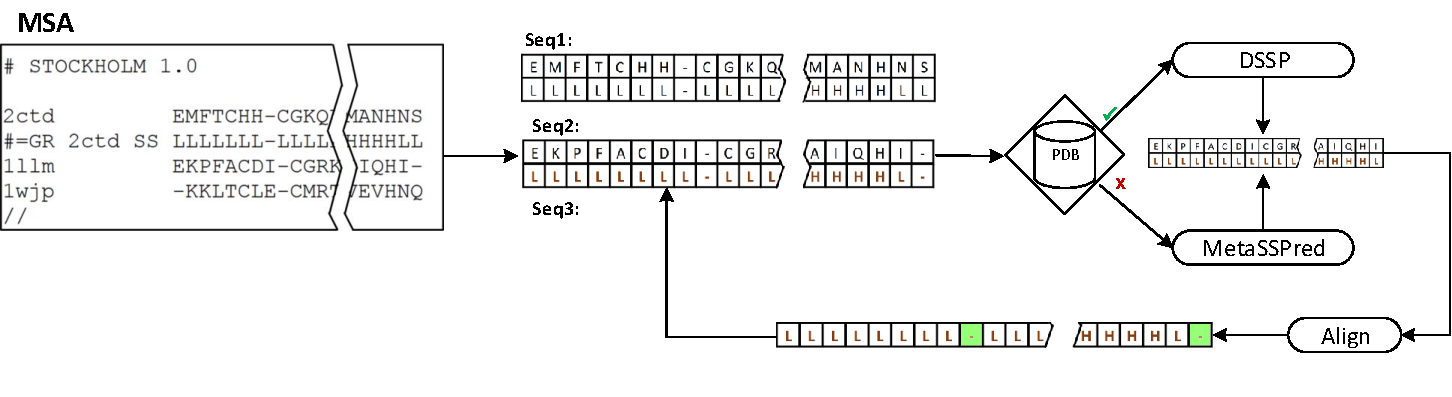
\includegraphics[width=\textwidth]{fig/ablaufMSA}
	\end{center}
	\caption[Workflow for processing input data.]{Workflow for processing input data and determination of secondary structure.}
	\label{fig:flowReadMSA}
\end{figure}

The secondary structure from sequences corresponding to three-dimensional data in the \ac{PDB} is calculated using the \ac{DSSP} program (see Section \ref{sec:DSSP}). The extracted structural information must be aligned with the original sequence, considering the exact gap positions and possible differences in the overall sequence length.  
The \mbox{Needleman--Wunsch} algorithm, described in \cite[p.\,19--21]{Durbin.1998}, is used for this task. 
Needleman--Wunsch is a dynamic programming approach for global sequence alignment that calculates the optimal path through a scoring matrix using match, mismatch, and gap penalties.
The derived sequences, linked to their corresponding secondary structure, are aligned with the original sequence. Provided the original sequence from the \ac{MSA} matches the aligned sequence from the \ac{PDB}, the determined secondary structure is used. 

If there is no match in the \ac{PDB} or the alignment fails, the secondary structure is predicted with MetaSSPred. For each sequence that must be predicted, a Fasta-formatted file with all gaps removed in the sequence is generated in the input directory of MetaSSPred and processed by the software. For the prediction process, ambiguous amino acids have to be treated separately, as most prediction methods including MetaSSPred only support the 20 common amino acids. Therefore, those symbols are also  removed for the prediction process. 
Subsequently, the symbol X is added at the removed position in the secondary structure data, which will be handled by HMModeler in the same way as all three secondary structure types.
Finally, the predicted secondary structure is aligned to the sequence with the Needleman--Wunsch algorithm. 

\section{Training the HMM}
\label{sec:training}

Based on the \ac{MSA}, which now includes both primary and secondary structures, the transitions and emission distribution are assigned to the \ac{pHMM}.
These are calculated by the frequencies across sequences for each column in the \ac{MSA}, according to (\ref{eq:transProb}), where $a_{kl}$ is the transition probability from state $k$ to $l$, and (\ref{eq:emission}) for the emission probability $e_k(a)$ of the symbol $a$ at state $k$. 

\begin{equation}
a_{kl} = \frac{A_{kl}}{\sum_{l'}A_{kl'}}
\label{eq:transProb}
\end{equation}

\begin{equation}
e_{k}(a) = \frac{E_k(a)}{\sum_{a'}E_k(a')}
\label{eq:emission}
\end{equation}

To prevent overfitting by symbols with a probability of zero, it is important to add some background frequency to each symbol, such as a small non-zero prior probability $pc(a)$ (see (\ref{eq:pseudo})). The simplest approach is the Laplace smoother, which adds a hypothetical observation in the form of one pseudo-count to each emission and transition.

\begin{equation}
e_{k}(a) = \frac{E_k(a) + pc(a)}{\sum_{a'}E_k(a') + \sum pc(a')}
\label{eq:pseudo}
\end{equation}


The implementation for the emission probabilities was extended by calculating the primary structure with 20+1 symbols to generate two additional matrices, one with 3+1 symbols for the secondary structure and another with 84 symbols containing mixed probabilities from the other two sets. The additional symbol for the primary and secondary structures was added to cover a wider set of sequences in the test database (see Section \ref{sec:TestData}), where single residues or structure elements in sequences may be unknown and therefore marked with the letter X. As the symbol X represents all other symbols in the set, the probability is set to 1. This is equal to the sum of all other probabilities. 


The transition probabilities only rely  on the gap positions of the \ac{MSA}. Therefore, no modifications in the current implementation of HMModeler are needed. Moreover, the functional emission probability implementation for the primary structure remains the same.

The emission probabilities for the secondary structure are calculated by using the three major types of helix, strand and loop. Therefore, secondary structure data from methods with higher granularity, such as \ac{DSSP}, are translated to the three-type annotation (see Table \ref{tab:DSSPStruct}). 
  To prevent zero probabilities, a prior probability can be set by the user in the HMModeler \ac{GUI}.

Using both probability sets, the original primary structure implementation and the new secondary structure probabilities, a weighted emission frequency set that covers both primary and secondary probabilities is generated. 
Mayer discusses the emission probability weighting for use with \ac{pHMM} in \cite{Mayer.2014}. Following his research, three different implementations are explained below.

\subsection{Linear Weighting}

In \cite{Mayer.2014}, Mayer discusses the problem with the different length of the two alphabets, as the primary structures involve 20 amino acid symbols and the secondary structure only involves three symbols. Therefore, he recommends  the approach in  (\ref{eq:mix1}), where the mixed emission probabilities $e_k(p,s)$ are weighted by their symbol length with 20 amino acids for the primary probability $e_k(p)$ and the three structure symbols in $e_k(s)$.   

\begin{equation}
e_k(p,s) = \frac{20}{20+3}\cdot e_k(p) + \frac{3}{20+3} \cdot e_k (s)
\label{eq:mix1}
\end{equation}


However, the most convenient approach for mixing two probabilities, which is by means of a simple multiplication as in  (\ref{eq:mix2}), will also be implemented and tested. 

\begin{equation}
e_k(p,s) =  e_k(p) \cdot e_k (s) \cdot k
\label{eq:mix2}
\end{equation}

As mentioned in Section \ref{sec:scoring} below, a threshold can be used to define whether  the scoring process uses the mixed or the primary  probability. The additional factor $k$ is introduced for scaling the resulting mixed probability. 
With this factor, the differences in the \ac{pHMM} resulting from the use of either mixed probability or primary probability can be reduced.


For example, if the three secondary structure elements are equally distributed with a probability of $e_k(s) = \frac{1}{3}$ and a $k=1$, the value of the mixed probability would also be $\frac{1}{3}$ of the value of the primary probability. By setting the factor $k=3$, an equally distributed secondary structure would not differ if the primary probability or the mixed probability were used.  

\subsection{Weighting by Shannon}


In \cite{Mayer.2014}, Mayer introduces weighting the two emission probabilities by the amount of information in each column using the Shannon theorem, defined in \cite{Shannon.1948} as 


\begin{equation}
	H = -\sum _{i=1}^{N} p_i \log _b p_i
	\label{eq:shannon1}
\end{equation}


where the entropy $H$ is the negative sum over the probability of each possible outcome $p_i$ multiplied by the logarithm of the same probability.
If a single probabilistic result of an event has a probability of $1$, the entropy is $0$. In this case, there is no uncertainty. Conversely, if all probabilistic results have equal probability, the uncertainty is maximal, with an entropy of $\log_b(N)$, where $N$ is the number of possible outcomes.  
The logarithmic base $b$ is usually $2$, as the common use is digital communication. In other cases, the natural logarithm $e$ is used. 

Figure \ref{fig:shannon} shows the entropy as a function for a binary event with probabilities $p$ and $q = 1-p$ with a natural logarithm and logarithmic base of 2. The maximum entropy occurs when $p=q=0.5$. 

\begin{figure}[ht]
	\begin{center}
		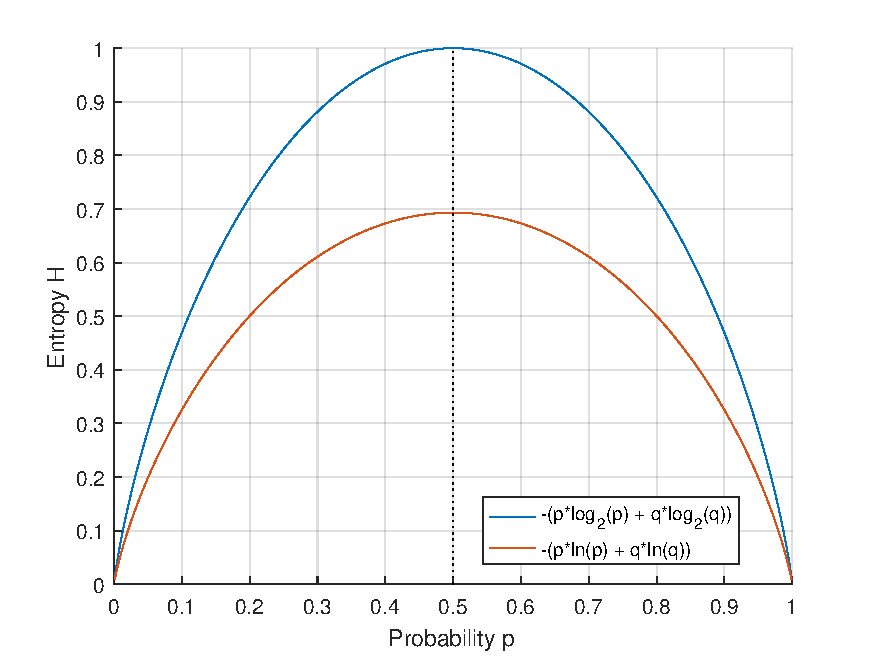
\includegraphics[width=0.8\textwidth]{fig/shannon}
	\end{center}
	\caption[Entropy H for an event with two possible outcomes.]{Entropy H for an event with two possible outcomes, with natural logarithm (red) and normalized logarithm with base 2 (blue).} 
	\label{fig:shannon}
\end{figure}


The lower the entropy, the higher the degree of information and thus the relevance of the mixed probability. The rate of information $I$ is determined by subtracting the entropy $H$ from the maximal possible entropy  $\log_b(N)$:

\begin{equation}
	I = \log_b(N)- H
\end{equation}

With the degree of information for both the primary structure $I(p)$ and the secondary structure $I(s)$, the  probabilities are weighted as follows:

\begin{equation}
	e_k(p,s) = \frac{I(p) \cdot e_k(p) + I(s) \cdot e_k(s)}{I(p)+I(s)}
	\label{eq:shannonfinal}
\end{equation}
 

Instead of using the natural logarithm for both the primary and secondary structure, as recommended by Mayer, the normalized logarithm with a base equal to the corresponding alphabet size is used in the present thesis. Without the normalization, the probabilities would not be equally weighted, as the maximum entropy for the  primary structure would be $ln(20)= 2.9957$ and for the secondary structure  $ ln(3) = 1.0986$. By contrast, the maximum entropy for both structures using the normalized logarithm is $\log_{3}(3)= \log_{20}(20) = 1$.

For programming languages that do not support nonstandard logarithmic bases, any logarithmic equation with base $a$ can be converted to any other base $b$ by dividing through the logarithm with the same base $a$, with the argument set to the new base $b$:


\begin{equation}
	\log_b(x) = \frac{\log_a(x)}{\log_a(b)}
	\label{eq:logBase}
\end{equation}
 
 
% #################################################################
%%---------------------------   SCORING     -----------------------
% #################################################################
\section{Scoring Sequences}
\label{sec:scoring}

HMModeler calculates nine different types of scores, (see Table \ref{tab:Hmscores}) using the Viterbi and forward algorithms. It also computes variations of these for length-corrected scores using the simple null model and the reversed sequence null model (see Section \ref{sec:scoringTh}). 

\begin{table}[h!]
\centering
\begin{tabular}{|l|l|}
\hline
Score type					& Description\\ \hline
Viterbi score                    & $\text{V}(s)$                         \\ 
Forward score                    & $\text{F}(s)$                         \\ 
Simple null model                & $\text{N}(s)$                         \\ 
Reverse Viterbi null model       & $\text{V}(s^{-1})$      \\ 
Reverse forward null model       & $\text{F}(s^{-1})$      \\ 
Simple corrected Viterbi score   & $\text{V}(s)-\text{N}(s)$                    \\ 
Simple corrected forward score   & $\text{F}(s)-\text{N}(s)$                    \\ 
Reverse corrected  Viterbi score & $\text{V}(s)-\text{V}(s^{-1})$ \\ 
Reverse corrected forward score \qquad & $\text{F}(s)-\text{F}(s^{-1})$   \qquad \\  \hline
\end{tabular}
\caption{Scores calculated by HMModeler.}
\label{tab:Hmscores}
\end{table}

Only the algorithms for the Viterbi score and the forward score must be adapted for the use of the secondary structure. The reversed null models for both the Viterbi and forward scores use the same underlying algorithm but with the sequence reversed. The simple null model uses a one-state \ac{HMM} with general background distribution based on the primary structure that  will continue to be used.


As described in Section \ref{sec:training}, the mixed emission probabilities $e_k(p,s)$ are generated based on the primary structure probabilities $e_k(p)$ and secondary structure probabilities $e_k(s)$. However, with the aim of using only the primary structure instead of the mixed probabilities for regions in the \ac{MSA} where the primary structure is highly conserved, a threshold can be set. If the highest emission probability in the primary structure is set below the threshold, the mixed probabilities are used. Otherwise, only the probabilities for the primary structure are used: 

\begin{equation}
e_k(m) =
  \begin{cases}
    e_k(p)  &  \text{if}\: \max(e_k(p')) > threshold \\
    e_k(p,s) & \text{otherwise}
  \end{cases}
  \label{eq:weighting}
\end{equation}

The resulting probability $e_k(m)$ will be used in the Viterbi equation for the transition to the match-state $V_j^M$:

\begin{equation}
V_k^M(k) = \log e_k(m)+ \text{max} 
\begin{cases}
V_{k-1}^M(i-1) + \log a_{M_{k-1} M_k}\\
V_{k-1}^I(i-1) + \log a_{I_{k-1} M_k}\\
V_{k-1}^D(i -1) + \log a_{D_{k-1} M_k} \\
V_{k-1}^{FB}{(i-1)} + \log a_{FB M_k}
\end{cases}
\label{eq:Viterbi}
\end{equation} 

The other Viterbi equations remain unchanged; as for insertion states in (\ref{eq:ViterbiInsert}), a background probability $q(p)$ based on the primary structure alphabet will be emitted, and the silent deletion states in (\ref{eq:ViterbiDeletion}) do not emit any symbol.

\begin{equation}
V_k^I(k) = \log q(p)+ \text{max} 
\begin{cases}
V_{k}^M(i-1) + \log a_{M_{k} D_k}\\
V_{k}^I(i-1) + \log a_{I_{k} D_k}\\
V_{k}^D(i-1) + \log a_{D_{k} D_k}
\end{cases}
\label{eq:ViterbiInsert}
\end{equation} 


\begin{equation}
V_k^D(k) = \text{max} \begin{cases}
V_{k-1}^M(i-1) + \log a_{M_{k-1} D_k}\\
V_{k-1}^I(i-1) + \log a_{I_{k-1} D_k}\\
V_{k-1}^D(i -1) + \log a_{D_{k-1} D_k} 
\end{cases}
\label{eq:ViterbiDeletion}
\end{equation} 


The same modification applies to the match state in the forward algorithm in (\ref{eq:ForwardMatch}), which is similar to the Viterbi algorithm. An exception is that instead of using the path with the maximum transition state, it sums up all transition states. 

\begin{equation}
\label{eq:ForwardMatch}
\begin{split}
F^M_k(i)= \log e_k(m) + \log&[  a_{M_{k-1}M_k} \: \exp(F_{k-1}^M(i-1))  \\
					 	  &+ a_{I_{k-1}M_k} \: \exp(F_{k-1}^I(i-1))		\\			 	  
					 	  &+ a_{D_{k-1}M_k} \: \exp(F_{k-1}^D(i-1))	\\
					 	  &+a_{FBM_k} \: \exp(F_{k-1}^{FB}(i-1))]
\end{split}
\end{equation}
